\section{Durchführung}
\label{sec:Durchführung}

\subsection{Versuchsaufbau}
\label{sec:Versuchsaufbau}
%\begin{figure}
%	\centering
%	\caption{Schematische Darstellung des Versuchsaufbaus \cite{anleitung}.}
%	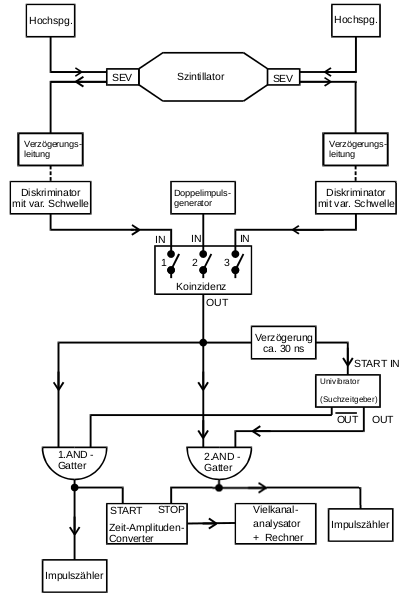
\includegraphics{Bilder/aufbau.png}
%	\label{fig:aufbau}
%\end{figure}
%
%\begin{figure}
%	\centering
%	\caption{Schematische Darstellung der Quelle zur Erzeugung radioaktiven Isotopen \cite{anleitung}.}
%	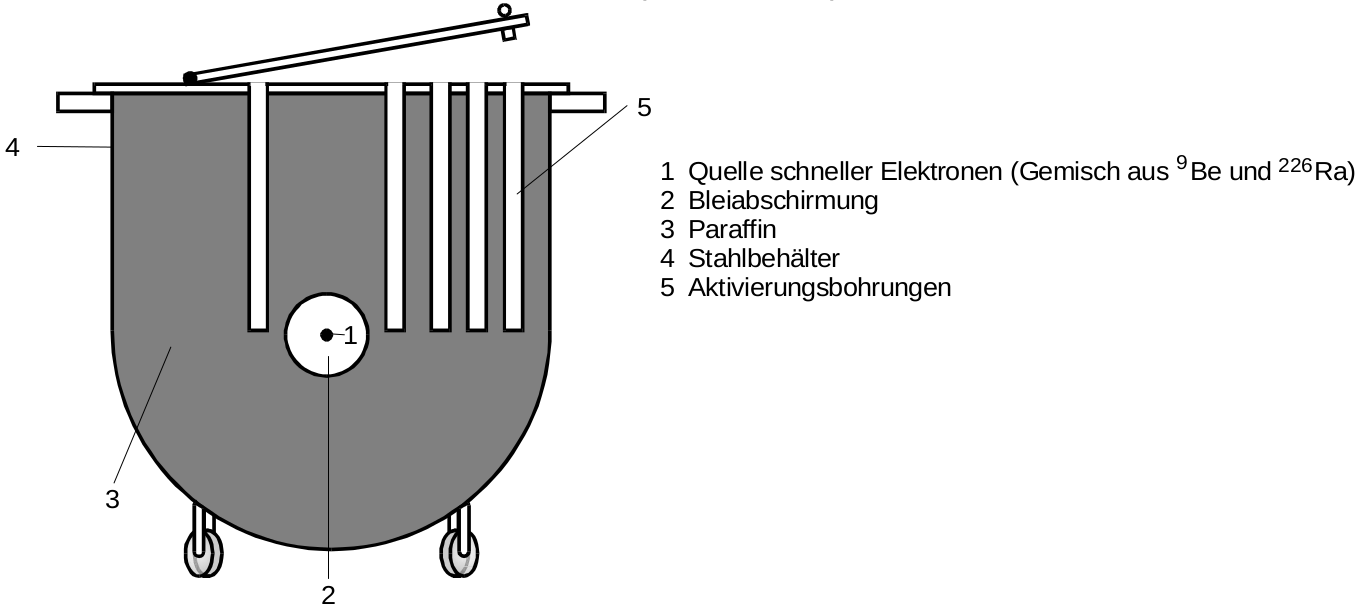
\includegraphics{content/toepfchen.png}
%	\label{fig:kochen}
%\end{figure}
%
Der Versuchsaufbau -- wie in Abbildung \ref{fig:aufbau} dargestellt -- besteht im Wesentlichen 
aus einem zerfallenden radioaktiven Isotop und einem Geiger-Müller-Zählrohr, welches die 
zerfallenden Kerne misst.
Das Geiger-Müller-Zählrohr ist entspricht einer mit Gas gefüllten Röhre. Trifft ein $\beta$-
oder $\gamma$- Teilchen auf ein Gasteilchen wird dieses ionisiert und kann aufgrund einer
anliegenden Spannung an der Röhre gemessen werden.
Dabei werden die gemessenen Zerfälle pro Messzeitintervall, welches am Zeitgeber einstellbar 
ist, an den Zählern 1 und 2 angezeigt. Nach jedem Messvorgang wird der Zähler umgeschaltet und 
der vorherige Wert auf dem aktuellen Zähler wird überschrieben. Der Versuchsaufbau ist mit
einer Blei-Abschirmung ausgestattet um die radioaktive Strahlung abzuschirmen.

Zur Erzeugung der radioaktiven Isotope wird das Objekt in Abbildung \ref{fig:kochen} verwendet.
Hierbei werden stabile Kerne mit niederenergetischen Neutronen beschossen. 
Da die Neutronen ihre Energie durch elastische Stöße an die Kerne übergeben und die maximale
Energie bei gleichen Massen der Stoßpartner erreicht wird, werden die Neutronen in einem 
Paraffinmantel gebremst, bis sie die optimale Energie besitzen.


\subsection{Versuchsbeschreibung}
\label{sec:Versuchsbeschreibung}
Vor Beginn der eigentlichen Untersuchung des Zeeman-Effekts muss der im Versuchsaufbau verwendete Elektromagnet zunächst geeicht werden.\\
Hierzu wird eine Hall-Sonde möglichst senkrecht in das B-Feld des Elektromagneten eingebracht und der Feldstrom in Schritten von $\SI{0.5}{\ampere}$ hochgeregelt und das zugehörige Magnetfeld in Abhängigkeit der Stromstärke notiert.
Anschließend wird der Versuchsaufbau wie in Abbildung \ref{fig:aufbau} gezeigt, aufgebaut. Lediglich der Polarisationsfilter wird noch nicht eingebaut, da dieser einen großen Teil der Intensität des Lichtstrahls herausfiltert und daher hinderlich beim Optimieren des Strahlenganges ist.\\
Um ein möglichst gutes Bild zu erhalten, wird zunächst die Position des Objektiv $O$ und der Linse $L1$ solange variiert, bis ein möglichst scharfes Lichtbündel auf den Spalt $S1$ abgebildet wird.\\
Die Linse $L2$ wiederum wird solange verschoben, bis ein möglichst paralleles Lichtbündel auf das Gradsichtprisma trifft.
Hierbei ist darauf zu achten, dass das Lichtbündel etwa so groß ist wie das Prisma ist, sodass möglichst wenig Intensität in der Optik verloren geht.\\
Die Linse $L3$ wird nun so eingestellt, dass auf den Spalt $S2$ ein scharfes Linienspektrum abgebildet wird. Mit dem Spalt $S2$ kann nun eine diskrete Linie des Spektrums ausgewählt werden und in die weitere Optik gelassen werden.\\
Begonnen wird mit der grünen Spektrallinie, diese entsteht aufgrund eines Quecksilberanteils in der Lampe und wird zur Kalibrierung des Messaufbaus genutzt, da das menschliche Auge für sie besonders empfindlich ist.\\
Mit der Linse $L4$ wird der Lichtstrahl schließlich auf das Eintrittsprisma der Lummer-Gehrcke-Platte fokussiert. Die Lummer-Gehrcke-Platte wird nun so ausgerichtet, dass ihre planparallelen Platten in einem möglichst spitzen Winkel zum Strahlengang stehen, damit eine hohe Auflösung erzielt werden kann.\\
Die Kamera wird zunächst auf den manuellen Modus geschaltet und jede Autofokus-Funktion deaktiviert.
Da die Kamera parallele Strahlen aufnehmen soll, muss ihr Zoom auf unendlich gestellt werden.\\
Es wird nun solange etwas an der Lummer-Gehrcke-Platte gedreht, bis ein gutes Bild auf dem Kamerabildschirm abgebildet wird.
Nun kann die eigentliche Messung des Zeeman-Effekts beginnen. Dafür wird der Polarisationsfilter an eine beliebige Stelle des Strahlengangs eingebracht (zum Beispiel direkt nach der Linse $L1$).\\
Durch ein leichtes Verdrehen der Linse $L3$ kann nun eine der zu untersuchenden Spektrallinien auf den Spalt $S2$ abgebildet. Dies hat gegenüber einer Verschiebung des Spalts den Vorteil, dass die dahinterliegende Optik nicht neu angepasst werden muss.
Für beide zu vermessenden Linien wird schließlich sowohl mindestens ein Bild ohne, als auch mindestens ein Bild mit eingeschalteten Magnetfeld für die jeweils gewünschte Polarisation gemacht.\\
Für jeden zu untersuchenden Übergang wird zunächst noch das aufgrund des Auflösungsvermögen der Lummer-Gehrcke-Platte minimal nötige Magnetfeld zur deutlichen Auflösung der Aufspaltung berechnet und im weiteren Verlauf jeweils passend eingestellt.
Da dies nicht für alle Übergänge mit dem vorliegenden Versuchsaufbau möglich ist, wird entsprechend das maximal mögliche Magnetfeld von etwa $\SI{1}{\tesla}$ eingestellt.\\
Für die rote Spektrallinie wird ein Bild ohne Magnetfeld und jeweils durch das Einstellen des Polarisators ein Bild nur mit zirkular und eins mit linear polarisierten Licht gespeichert.\\
Für die Untersuchung der blauen Spektrallinie wird analog vorgegangen.\\
Es empfiehlt sich für jede Messung nicht nur ein Bild zu speichern, sondern jeweils eine Bildserie mit verschiedenen Belichtungszeiten und ISO-Werten aufzunehmen um möglichst gute Bilder zu erhalten.
